\chapter{Re\c{t}ele neuronale convolu\c{t}ionale}

Re\c{t}elele neuronale convolutionale folosesc trei idei de baz\i{a} : local receptive fields, shared weights \c{s}i pooling.

\par

Local receptive fields : in loc sa mai luam fiecare valoare a unui pixel separat \c{s}i s\u{a} o introducem intr-un neuron de pe un nivel intermediar ( hidden layer ) ca dat\u{a} de intrare putem s\u{a} grup\u{a}m pixelii in blocuri de pixeli \c{s}i s\u{a} \^{i}i trimitem grupa\c{t}i la un neuron de pe primul nivel intermediar ( hidden layer ).   Cum se observ\u{a} \c{s}i \^{i}n imaginea de mai jos, un grup de 5 x 5 pixeli este trimis grupat c\u{a}tre un singru neuron de pe primul nivel intermediar.

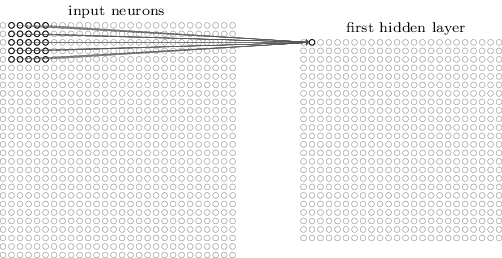
\includegraphics[width=300]{conv.png}

Fieacre bloc de pixeli are c\^{a}te o greutate ( weights ), iar neuronul de pe nivelul intermediar care prime\c{s}te acest bloc de pixeli ca dat\u{a} de intreare are un bias / un trashold.

\par

Dac\u{a} spargem o imagine de 28 x 28 pixeli in blocuri de 5 x 5 pixeli \c{s}i ne mi\c{s}c\u{a}m cu un pixel la dreapta sau in jos pentru fiecare bloc de pixeli pe care vrem s\u{a} \^{i}l extragem, atunci pe primul nivel intermediar vom avea 24 x 24 de valori.

\par

Shared weights and biases : se va folosii acela\c{s} weights si bias pentru fiecare neuron de pe primul nivel intermediar.

\par

Pooling layers: nivelul de pooling se pune intre doua nivele convolutionale pentru a se reduce cantitatea de informa\c{t}ie care se duce c\u{a}tre urm\u{a}torul nivel convolutional. Cel mai folosit tip de pooling este max-pooling care prime\c{s}te ca date de intrare valorile rezultate de la precedentul nivel convolutional \c{s}i le las\u{a} s\u{a} treac\u{a} doar pe cel cu valoarea cea mai mare catre urmatorul nivel convolutional ( vede\c{t}i imaginea de mai jos ), astfle c\u{a} acest nivel ne ajut\u{a} s\u{a} reducem cantitatea de date \c{s}i s\u{a} sc\u{a}p\u{a}m de datele nerelevante dintr-o re\c{t}ea convolutional\u{a}.

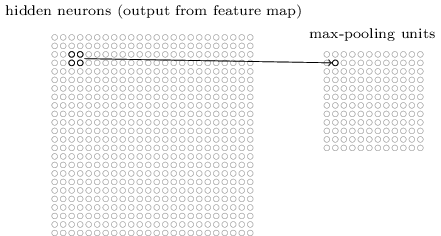
\includegraphics[width=300]{pool.png}

Cum se observ\u{a} \^{i}n imaginea de mai sus, nivelul de max-pooling prime\c{s}te patru valori de pe nivelul preceden \c{s}i las\u{a} o singur\u{a} valoarea s\u{a} treac\u{a} mai departe.